\documentclass{article}

\usepackage{fullpage}
\usepackage{graphicx}
\usepackage{color}
\usepackage{fancyhdr}
\usepackage{url}
\usepackage{subfig}
\usepackage{amsmath,bm}
\usepackage{amssymb}
\usepackage{amsthm}
\usepackage{amsfonts}
\usepackage[round]{natbib}
\usepackage{enumitem,xcolor}
\usepackage[multiple]{footmisc}

\usepackage[
 pdftitle={Capstone Report - Udacity Machine Learning Nanodegree},
 pdfsubject={Machine Learning, Reinforcement Learning, Deep Learning, Artificial Intelligence, Games},
 pdfauthor={David Robles},
 pdfpagemode=UseOutlines,
 pdfborder= {0 0 1.0},
 bookmarks,
 bookmarksopen,
 colorlinks=true,
 citecolor=blue,
 linkcolor=blue, %
 linkbordercolor=blue, %
 urlcolor=blue, %
]{hyperref}

\usepackage[labelfont=bf]{caption}


\usepackage[utf8]{inputenc}

% Default fixed font does not support bold face
\DeclareFixedFont{\ttb}{T1}{txtt}{bx}{n}{8} % for bold
\DeclareFixedFont{\ttm}{T1}{txtt}{m}{n}{8}  % for normal

% Custom colors
\usepackage{color}
\definecolor{deepblue}{rgb}{0,0,0.5}
\definecolor{deepred}{rgb}{0.6,0,0}
\definecolor{deepgreen}{rgb}{0,0.5,0}

\usepackage{listings}

\definecolor{codebg}{RGB}{238,238,238}

% Python style for highlighting
\newcommand\pythonstyle{\lstset{
language=Python,
basicstyle=\ttm,
otherkeywords={self},             % Add keywords here
keywordstyle=\ttb\color{deepblue},
emph={MyClass,__init__},          % Custom highlighting
emphstyle=\ttb\color{deepred},    % Custom highlighting style
stringstyle=\color{deepgreen},
frame=tb,                         % Any extra options here
framesep=10pt,
framexleftmargin=10pt,
backgroundcolor=\color{codebg},
rulecolor=\color{codebg},
aboveskip=15pt,
belowskip=15pt,
showstringspaces=false            % 
}}


% Python environment
\lstnewenvironment{python}[1][]
{
\pythonstyle
\lstset{#1}
}
{}

% Python for external files
\newcommand\pythonexternal[2][]{{
\pythonstyle
\lstinputlisting[#1]{#2}}}

% Python for inline
\newcommand\pythoninline[1]{{\pythonstyle\lstinline!#1!}}

%%%%%%%%%%%%%%%%%%%%%%%%%%%%%%%%%%%%%%%%%%%%%%%%%%%%%%%%%%%%%%%%%%%%%%%%%%%%%%%%%%%%%%%%%%%%%%%%%%%%
\title{Machine Learning Nanodegree \\ Capstone Report}
\author{David A. Robles}
\date{January 31, 2017}
\begin{document}
\maketitle
%%%%%%%%%%%%%%%%%%%%%%%%%%%%%%%%%%%%%%%%%%%%%%%%%%%%%%%%%%%%%%%%%%%%%%%%%%%%%%%%%%%%%%%%%%%%%%%%%%%%

%%%%%%%%%%%%%%%%%%%%%%%%%%%%%%%%%%%%%%%%%%%%%%%%%%%%%%%%%%%%%%%%%%%%%%%%%%%%%%%%%%%%%%%%%%%%%%%%%%%%
\section{Definition}
%%%%%%%%%%%%%%%%%%%%%%%%%%%%%%%%%%%%%%%%%%%%%%%%%%%%%%%%%%%%%%%%%%%%%%%%%%%%%%%%%%%%%%%%%%%%%%%%%%%%

\subsection{Project Overview}

Content.

%%%%%%%%%%%%%%%%%%%%%%%%%%%%%%
\subsection{Problem Statement}
\label{sec:problem-statement}
%%%%%%%%%%%%%%%%%%%%%%%%%%%%%%

\newcommand{\URLcf}{https://en.wikipedia.org/wiki/Connect_Four}

In this project, we will use reinforcement learning with deep learning to make an agent learn to
play the game of {Connect 4}\footnote{\url{\URLcf}} by playing games against itself. In other words,
using the formalism used by \cite{Mitchell1997Book} to define a machine learning problem:

\begin{itemize}

    \item \textbf{Task:} Playing Connect 4.

    \item \textbf{Performance:} Percent of games won against other agents, and accuracy of the
        predictions on a Connect 4 dataset.

    \item \textbf{Experience:} Games played against itself.

    \item \textbf{Target function:} $Q^\pi : \mathcal{S} \times \mathcal{A} \to \mathbb{R}$, where
        $\mathcal{S}$ is the set of \emph{states} (board positions) and $\mathcal{A}$ is the set of
        \emph{actions} (moves), and $\mathbb{R}$ represents the value of being in a state $s \in
        \mathcal{S}$, applying a action $a \in \mathcal{A}$, and following policy $\pi$ thereafter.

    \item \textbf{Target function representation:} Deep neural network.

\end{itemize}

Therefore, I seek to build a Q-learning agent trained via a deep convolutional neural network to
approximate the optimal action-value function:

\begin{equation}
Q^*(s,a) = \max\limits_\pi Q^\pi(s,a), \forall s \in \mathcal{S}, a \in \mathcal{A}
\end{equation}

\noindent which is the maximum sum of rewards achievable by a behaviour policy $\pi$.

%%%%%%%%%%%%%%%%%%%%
\subsection{Metrics}
%%%%%%%%%%%%%%%%%%%%

\begin{itemize}

    \item \textbf{Winning percentage.} This metric consists in playing a high number of games (e.g.
        100,000) against another agent (e.g. a random agent), and calculating the average of games
        won by the agent that uses the learned value function.
        
    \item \textbf{Prediction accuracy.} The learned value function will be used to predict the
        game-theoretic outcomes (win, loss or draw) of the board positions in the Connect 4 Data
        Set.

\end{itemize}

%%%%%%%%%%%%%%%%%%%%%%%%%%%%%%%%%%%%%%%%%%%%%%%%%%%%%%%%%%%%%%%%%%%%%%%%%%%%%%%%%%%%%%%%%%%%%%%%%%%%
\section{Analysis}
%%%%%%%%%%%%%%%%%%%%%%%%%%%%%%%%%%%%%%%%%%%%%%%%%%%%%%%%%%%%%%%%%%%%%%%%%%%%%%%%%%%%%%%%%%%%%%%%%%%%

\subsection{Data Exploration}

Content.

\subsection{Exploratory Visualization}

Content.

\subsection{Algorithms and Techniques}

\subsubsection{Q-learning}

One of the most basic and popular methods to estimate action-value functions is the
\emph{Q-learning} algorithm~\citep{Watkins1989PhD}. It is model-free online off-policy algorithm,
whose main strength is that it is able to compare the expected utility of the available actions
without requiring a model of the environment. Q-learning works by learning an action-value function
that gives the expected utility of taking a given action in a given state and following a fixed
policy thereafter. The update rule uses action-values and a built-in max-operator over the
action-values of the next state in order to update $Q(s_t, a_t)$ as follows,
%
\begin{equation}
    Q(s_t, a_t) \gets Q(s_t, a_t) + \alpha [r_{t+1} + \gamma \max_a Q(s_{t+1}, a) - Q(s_t, a_t)]
\end{equation}

The agent makes a step in the environment from state $s_t$ to $s_{t+1}$ using action $a_t$ while
receiving reward $r_t$. The update takes place on the action-value $a_t$ in the state $s_t$ from
which this action was executed.

Q-learning is exploration-intensive, which means that it will converge to the optimal policy
regardless of the exploration policy being followed, under the assumption that each state-action
pair is visited an infinite number of times, and the learning parameter $\alpha$ is decreased
appropriately~\citep{Watkins1992Q}.

\subsubsection{Self-play}

Self-play is by far the most popular training method. It is a single policy $\pi(s,a)$ that is used
by both players in a two-player game, $\pi_1(s,a) = \pi_2(s,a) = \pi(s,a)$. The first reason for its
popularity is that training is quickest if the learner's opponent is roughly equally strong, and
that definitely holds for self-play. As a second reason for popularity, there is no need to
implement or access a different agent with roughly equal playing strength. However, self-play has
several drawbacks, with the main one being that a single opponent does not provide sufficient
exploration~\citep{Szita2011RLGames}.

\subsection{Benchmark}

Content.

%%%%%%%%%%%%%%%%%%%%%%%%%%%%%%%%%%%%%%%%%%%%%%%%%%%%%%%%%%%%%%%%%%%%%%%%%%%%%%%%%%%%%%%%%%%%%%%%%%%%
\section{Methodology}
%%%%%%%%%%%%%%%%%%%%%%%%%%%%%%%%%%%%%%%%%%%%%%%%%%%%%%%%%%%%%%%%%%%%%%%%%%%%%%%%%%%%%%%%%%%%%%%%%%%%

\subsection{Data Preprocessing}

Content.

\subsection{Implementation}

- Two games were implemented: Tic Tac Toe and Connect 4.
- Converting a to an MDP by using a fixed agent.
- Show that q-learning learns to play against a fixed opponent using Tic-Tac-Toe.
- Show that q-learning learns to play against a fixed opponent using Connect 4.

\subsection{Refinement}

Content.

%%%%%%%%%%%%%%%%%%
\subsection{Games}
%%%%%%%%%%%%%%%%%%

%%%%%%%%%%%%%%%%%%%%%%%%%%%
\subsubsection{Tic Tac Toe}
%%%%%%%%%%%%%%%%%%%%%%%%%%%

Content.

%%%%%%%%%%%%%%%%%%%%%%%%%
\subsubsection{Connect 4}
%%%%%%%%%%%%%%%%%%%%%%%%%

Connect 4 is a two-player board game of perfect information where pieces are dropped into the
columns of a vertical $6 \times 7$ grid with the goal of forming a straight line of 4 connected
pieces. There are at most 7 actions per state, since placing a piece in a column is a legal action
only if that column has at least one empty location. \hyperref[fig:c4-game]{Figure~\ref*{fig:c4-game}}
shows three Connect 4 game positions. 

%%%%%%%%%%
% Figure %
%%%%%%%%%%

\begin{figure}[!h]
    \centering
    \subfloat[Win for \textsc{Player 1}]{
        \label{fig:c4-game-1}
        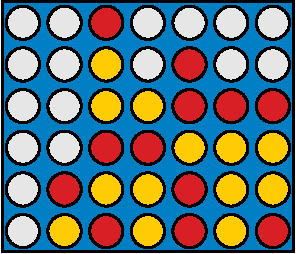
\includegraphics[width=0.25\textwidth]{figures/c4/c4-win-blue-c5f2.pdf}
    } \hspace{0.2in}
    \subfloat[Win for \textsc{Player 2}]{
        \label{fig:c4-game-2}
        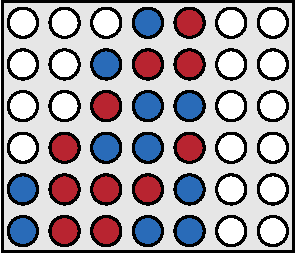
\includegraphics[width=0.25\textwidth]{figures/c4/c4-win-red-b3e6.pdf}
    } \hspace{0.2in}
    \subfloat[Draw]{
        \label{fig:c4-game-3}
        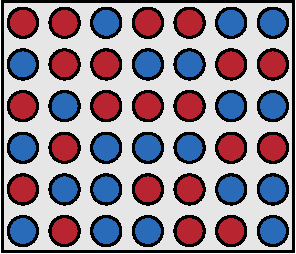
\includegraphics[width=0.25\textwidth]{figures/c4/c4-draw.pdf}
    }
    \caption{Examples of wins, losses and draws in Connect Four}
    \label{fig:c4-game}
\end{figure}

%%%%%%%%%%%%%%%%%%%%%%%%%%%%%%%%%%%%%%%%%%%%%%%%%%%%%%%%%%%%%%%%%%%%%%%%%%%%%%%%%%%%%%%%%%%%%%%%%%%%
\section{Results}
%%%%%%%%%%%%%%%%%%%%%%%%%%%%%%%%%%%%%%%%%%%%%%%%%%%%%%%%%%%%%%%%%%%%%%%%%%%%%%%%%%%%%%%%%%%%%%%%%%%%

\subsection{Model Evaluation and Validation}

Content.

\subsection{Justification}

Content.

%%%%%%%%%%%%%%%%%%%%%%%%%%%%%%%%%%%%%%%%%%%%%%%%%%%%%%%%%%%%%%%%%%%%%%%%%%%%%%%%%%%%%%%%%%%%%%%%%%%%
\section{Conclusion}
%%%%%%%%%%%%%%%%%%%%%%%%%%%%%%%%%%%%%%%%%%%%%%%%%%%%%%%%%%%%%%%%%%%%%%%%%%%%%%%%%%%%%%%%%%%%%%%%%%%%

\subsection{Free-Form Visualization}

Content.

\subsection{Reflection}

Content.

\subsection{Improvement}

Content.

%%%%%%%%%%%%%%%%%%%%%%%%%%%%%%%%%%%%%%%%%%%%%%%%%%%%%%%%%%%%%%%%%%%%%%%%%%%%%%%%%%%%%%%%%%%%%%%%%%%%
% BIBLIOGRAPHY
%%%%%%%%%%%%%%%%%%%%%%%%%%%%%%%%%%%%%%%%%%%%%%%%%%%%%%%%%%%%%%%%%%%%%%%%%%%%%%%%%%%%%%%%%%%%%%%%%%%%

\bibliographystyle{plainnat}
\bibliography{bibliography}

\end{document}
